
\documentclass[10pt]{article}

\usepackage[a4paper,margin=0.65in]{geometry}
\usepackage{amsmath,amssymb}
\usepackage{graphicx}
\usepackage{booktabs}
\usepackage{array}
\usepackage{float}
\usepackage{hyperref}
\usepackage{enumitem}
\usepackage{xcolor}
\usepackage{tikz}
\usetikzlibrary{positioning,arrows.meta,shapes.geometric,fit,calc}

\setlist{nosep,leftmargin=*}
\renewcommand{\arraystretch}{1.2}
\setlength{\parindent}{0pt}
\setlength{\parskip}{2pt}

\tikzset{
layer/.style={
draw,
rounded corners,
minimum width=1.7cm,
minimum height=0.65cm,
align=center,
fill=blue!10,
font=\scriptsize
},
smalllayer/.style={
draw,
rounded corners,
minimum width=1.35cm,
minimum height=0.58cm,
align=center,
fill=green!10,
font=\scriptsize
},
arrow/.style={
-{Latex[length=2mm]},
thin
}
}

\begin{document}

%%%%%%%%%%%%%%%%%%%%%%%%%%%%%%%%%%%%%%%%%%%%%%%%%%%%%%%%%%%%
% TITLE
%%%%%%%%%%%%%%%%%%%%%%%%%%%%%%%%%%%%%%%%%%%%%%%%%%%%%%%%%%%%

\begin{center}

{\large\textbf{Shiv Nadar University Chennai}}

\vspace{2mm}

{\normalsize\textbf{CS3807 -- Deep Learning Laboratory}}

\vspace{2mm}

{\large\textbf{Experiment 7}}

\vspace{1mm}

{\normalsize\textbf{End-to-End Study of Autoencoders, Convolutional}}

{\normalsize\textbf{Autoencoders, Denoising Autoencoders and Variational Autoencoders}}


\noindent
\renewcommand{\arraystretch}{1.25}

\begin{tabular}{|p{3cm}|p{8cm}|p{2cm}|}
\hline
Degree \& Branch & B.Tech Artificial Intelligence \& Data Science & Semester V\\ \hline
Subject Code \& Name,Details & CS3807 -- Deep Learning Laboratory \hspace{2 cm} Kalpana Bhaskar (AI-DS:A, Roll no: 24011101049) & AY: 2026--27\\ \hline
\end{tabular}
\end{center}
%%%%%%%%%%%%%%%%%%%%%%%%%%%%%%%%%%%%%%%%%%%%%%%%%%%%%%%%%%%%
\section*{1. Objective}

The objective of this experiment is to develop an end-to-end understanding of
autoencoders and their variants for image representation, reconstruction,
denoising and generative modeling.

The experiment begins with a fully connected autoencoder, progresses to a
Convolutional Autoencoder (CAE), introduces image corruption for denoising,
and finally develops a Variational Autoencoder (VAE). Students will visualize
the learned latent representation, compare reconstruction quality using
quantitative and qualitative measures, and explore the generative capability
of the VAE.

The same image dataset and a controlled experimental protocol should be used
throughout the experiment wherever possible.

%%%%%%%%%%%%%%%%%%%%%%%%%%%%%%%%%%%%%%%%%%%%%%%%%%%%%%%%%%%%
\section*{2. Learning Outcomes}

After completing this experiment, students will be able to:

\begin{itemize}
\item explain the encoder--latent--decoder structure of an autoencoder;
\item prepare image data for reconstruction-based learning;
\item implement a fully connected autoencoder;
\item implement a Convolutional Autoencoder for image reconstruction;
\item introduce controlled noise and build a denoising autoencoder;
\item evaluate reconstruction using MSE, MAE and SSIM;
\item visualize and interpret latent representations;
\item explain the probabilistic latent representation of a VAE;
\item implement the reparameterization trick;
\item calculate and interpret reconstruction and KL-divergence losses;
\item generate new images by sampling from a learned latent space; and
\item compare deterministic and variational latent representations.
\end{itemize}

%%%%%%%%%%%%%%%%%%%%%%%%%%%%%%%%%%%%%%%%%%%%%%%%%%%%%%%%%%%%
\section*{3. Dataset and Experimental Setup}

\textbf{Dataset: MNIST Handwritten Digit Dataset}

MNIST contains grayscale images of handwritten digits from 0 to 9. Each image
has spatial dimensions

\[
28\times28\times1.
\]

The dataset is particularly suitable for this experiment because the images
are small, the classes have visually meaningful structure, and the same image
format can be directly supplied to fully connected, convolutional and
variational autoencoders.

The dataset can be loaded directly using Keras/TensorFlow:

\url{https://www.tensorflow.org/api_docs/python/tf/keras/datasets/mnist}

\textbf{Recommended laboratory subset:}

Use 10,000 training images and 2,000 test images for the main laboratory
execution. The full MNIST dataset may be used if computational resources
permit.

The labels are not required as reconstruction targets. The original image is
the target:

\[
\boxed{x\rightarrow \text{Encoder}\rightarrow z
\rightarrow\text{Decoder}\rightarrow\hat{x}}
\]

where $x$ is the input image and $\hat{x}$ is its reconstruction.

%%%%%%%%%%%%%%%%%%%%%%%%%%%%%%%%%%%%%%%%%%%%%%%%%%%%%%%%%%%%
\section*{4. Expected Input and Output}

\subsection*{Expected Input}

Each input image has shape

\[
28\times28\times1.
\]

For a batch of 32 images:

\[
X\in\mathbb{R}^{32\times28\times28\times1}.
\]

Pixel values should be converted from

\[
[0,255]\rightarrow[0,1].
\]

For a fully connected autoencoder, the image may be flattened:

\[
28\times28=784.
\]

Therefore,

\[
x\in\mathbb{R}^{784}.
\]

For a convolutional autoencoder, retain the spatial structure:

\[
x\in\mathbb{R}^{28\times28\times1}.
\]

\subsection*{Expected Output}

The primary output is a reconstructed image:

\[
\hat{x}\in\mathbb{R}^{28\times28\times1}.
\]

Students must display:

\begin{verbatim}
Original image
Reconstructed image
Reconstruction error
\end{verbatim}

For the denoising model, display:

\begin{verbatim}
Original clean image
Noisy image
Denoised reconstruction
\end{verbatim}

For the VAE, display newly generated samples obtained by sampling from the
latent distribution.

%%%%%%%%%%%%%%%%%%%%%%%%%%%%%%%%%%%%%%%%%%%%%%%%%%%%%%%%%%%%
\section*{5. Overall Experimental Pipeline}

The complete experiment follows:

\begin{center}
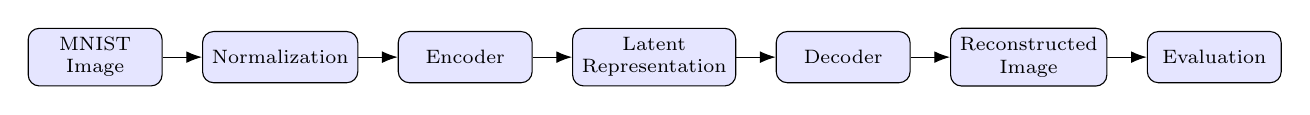
\begin{tikzpicture}[node distance=5mm]
\node[layer](a){MNIST\\Image};
\node[layer,right=of a](b){Normalization};
\node[layer,right=of b](c){Encoder};
\node[layer,right=of c](d){Latent\\Representation};
\node[layer,right=of d](e){Decoder};
\node[layer,right=of e](f){Reconstructed\\Image};
\node[layer,right=of f](g){Evaluation};

\foreach \x/\y in {a/b,b/c,c/d,d/e,e/f,f/g}
\draw[arrow](\x)--(\y);
\end{tikzpicture}
\end{center}

The experiment consists of four related studies:

\begin{enumerate}
\item Fully Connected Autoencoder
\item Convolutional Autoencoder
\item Denoising Convolutional Autoencoder
\item Variational Autoencoder
\end{enumerate}

%%%%%%%%%%%%%%%%%%%%%%%%%%%%%%%%%%%%%%%%%%%%%%%%%%%%%%%%%%%%
\section*{6. Exploring Autoencoders}

An autoencoder learns to reproduce its input at the output.

The encoder maps the input to a lower-dimensional representation:

\[
z=f_{\theta}(x),
\]

and the decoder reconstructs the input:

\[
\hat{x}=g_{\phi}(z).
\]

The training objective is to minimize reconstruction error:

\[
\mathcal{L}_{rec}
=
\frac{1}{N}\sum_{i=1}^{N}
\|x_i-\hat{x}_i\|^2.
\]

\begin{center}
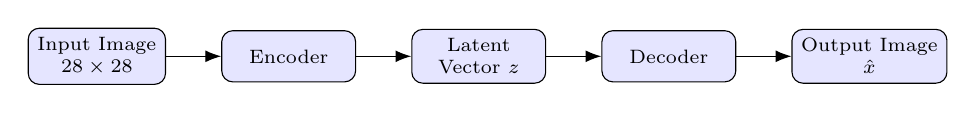
\begin{tikzpicture}[node distance=7mm]
\node[layer](a){Input Image\\$28\times28$};
\node[layer,right=of a](b){Encoder};
\node[layer,right=of b](c){Latent\\Vector $z$};
\node[layer,right=of c](d){Decoder};
\node[layer,right=of d](e){Output Image\\$\hat{x}$};

\foreach \x/\y in {a/b,b/c,c/d,d/e}
\draw[arrow](\x)--(\y);
\end{tikzpicture}
\end{center}

The latent vector is a compressed representation of the input.

%%%%%%%%%%%%%%%%%%%%%%%%%%%%%%%%%%%%%%%%%%%%%%%%%%%%%%%%%%%%
\section*{7. Fully Connected Autoencoder}

Flatten each image from

\[
28\times28=784
\]

to a vector of length 784.

Use the following architecture:

\begin{center}
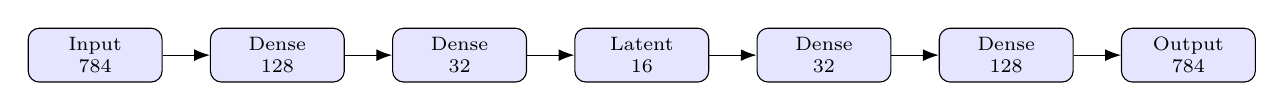
\begin{tikzpicture}[node distance=6mm]
\node[layer](a){Input\\784};
\node[layer,right=of a](b){Dense\\128};
\node[layer,right=of b](c){Dense\\32};
\node[layer,right=of c](d){Latent\\16};
\node[layer,right=of d](e){Dense\\32};
\node[layer,right=of e](f){Dense\\128};
\node[layer,right=of f](g){Output\\784};

\foreach \x/\y in {a/b,b/c,c/d,d/e,e/f,f/g}
\draw[arrow](\x)--(\y);
\end{tikzpicture}
\end{center}

Use ReLU activation in hidden layers and sigmoid activation in the output
layer.

\textbf{Suggested configuration:}

\begin{center}
\begin{tabular}{|l|l|}
\hline
Parameter & Value\\
\hline
Latent dimension & 16\\
Optimizer & Adam\\
Learning rate & $10^{-3}$\\
Batch size & 128\\
Epochs & 20\\
Loss & Binary Cross-Entropy\\
\hline
\end{tabular}
\end{center}

%%%%%%%%%%%%%%%%%%%%%%%%%%%%%%%%%%%%%%%%%%%%%%%%%%%%%%%%%%%%
\section*{8. Required Analysis of the Basic Autoencoder}

\textbf{Plot 1: Original versus Reconstructed Images}

Display at least 10 test images in a grid.

For every image, show:

\[
\text{Original}\quad|\quad\text{Reconstruction}.
\]

Students must comment on:

\begin{itemize}
\item preservation of digit shape;
\item loss of fine details;
\item blurred regions;
\item differences between easy and difficult samples.
\end{itemize}

\textbf{Plot 2: Training and Validation Reconstruction Loss}

\begin{itemize}
\item X-axis: Epoch
\item Y-axis: Reconstruction loss
\item Curves: Training loss and validation loss
\end{itemize}

\textbf{Required inference:} Determine whether the model converges and whether
there is evidence of overfitting.

%%%%%%%%%%%%%%%%%%%%%%%%%%%%%%%%%%%%%%%%%%%%%%%%%%%%%%%%%%%%
\section*{9. Reconstruction Metrics}

Students must calculate the following metrics on the test set.

\subsection*{Mean Squared Error}

\[
MSE=
\frac{1}{N}
\sum_{i=1}^{N}
(x_i-\hat{x}_i)^2.
\]

\subsection*{Mean Absolute Error}

\[
MAE=
\frac{1}{N}
\sum_{i=1}^{N}
|x_i-\hat{x}_i|.
\]

\subsection*{Structural Similarity}

Calculate SSIM between the original and reconstructed images.

The implementation may use:

\url{https://scikit-image.org/docs/stable/api/skimage.metrics.html}

Report:

\begin{center}
\begin{tabular}{|l|c|}
\hline
Metric & Value\\
\hline
Test MSE & 0.001926\\
Test MAE & 0.012844\\
Mean SSIM & 0.9812\\
Parameters & 74497\\
\hline
\end{tabular}
\end{center}

%%%%%%%%%%%%%%%%%%%%%%%%%%%%%%%%%%%%%%%%%%%%%%%%%%%%%%%%%%%%
\section*{10. Convolutional Autoencoder}

A Convolutional Autoencoder preserves spatial structure and uses convolutional
operations in the encoder and upsampling/transposed convolution operations
in the decoder.

The conceptual architecture is:

\begin{center}
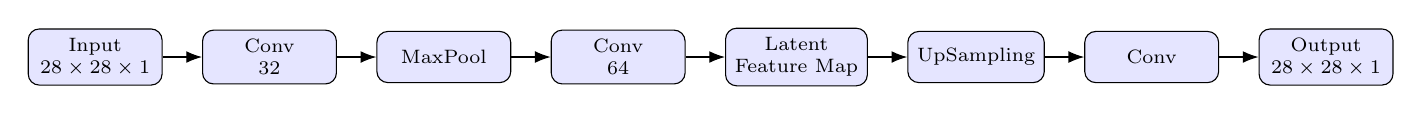
\begin{tikzpicture}[node distance=5mm]
\node[layer](a){Input\\$28\times28\times1$};
\node[layer,right=of a](b){Conv\\32};
\node[layer,right=of b](c){MaxPool};
\node[layer,right=of c](d){Conv\\64};
\node[layer,right=of d](e){Latent\\Feature Map};
\node[layer,right=of e](f){UpSampling};
\node[layer,right=of f](g){Conv};
\node[layer,right=of g](h){Output\\$28\times28\times1$};

\foreach \x/\y in {a/b,b/c,c/d,d/e,e/f,f/g,g/h}
\draw[arrow](\x)--(\y);
\end{tikzpicture}
\end{center}

A possible implementation is:

\begin{verbatim}
Input(28,28,1)
Conv2D(32, 3, activation='relu', padding='same')
MaxPooling2D(2, padding='same')
Conv2D(64, 3, activation='relu', padding='same')
MaxPooling2D(2, padding='same')
Conv2D(64, 3, activation='relu', padding='same')
UpSampling2D(2)
Conv2D(32, 3, activation='relu', padding='same')
UpSampling2D(2)
Conv2D(1, 3, activation='sigmoid', padding='same')
\end{verbatim}

The exact implementation may use Conv2DTranspose instead of UpSampling2D.

%%%%%%%%%%%%%%%%%%%%%%%%%%%%%%%%%%%%%%%%%%%%%%%%%%%%%%%%%%%%
\section*{11. Comparing Fully Connected and Convolutional Autoencoders}

Train both models using the same training and test images.

\begin{center}
\begin{tabular}{|l|c|c|c|c|}
\hline
Model & MSE & MAE & SSIM & Parameters \\
\hline
Fully Connected AE & 0.023641 & 0.061607 & 0.720087 & 211040 \\
Convolutional AE   & 0.001926 & 0.012844 & 0.981171 & 74497  \\
\hline
\end{tabular}
\end{center}

\textbf{Plot 3: Reconstruction Comparison}

Display:

\[
\text{Original}
\rightarrow
\text{FC-AE Reconstruction}
\rightarrow
\text{CAE Reconstruction}.
\]

\textbf{Required inference:}

Discuss how preserving spatial locality through convolution affects image
reconstruction.

%%%%%%%%%%%%%%%%%%%%%%%%%%%%%%%%%%%%%%%%%%%%%%%%%%%%%%%%%%%%
\section*{12. Denoising Autoencoder}

A denoising autoencoder receives a corrupted image but is trained to
reconstruct the original clean image.

The training mapping is:

\[
\boxed{\tilde{x}\rightarrow\text{Encoder}\rightarrow z
\rightarrow\text{Decoder}\rightarrow\hat{x}}
\]

where $\tilde{x}$ is a noisy version of the clean image $x$.

\begin{center}
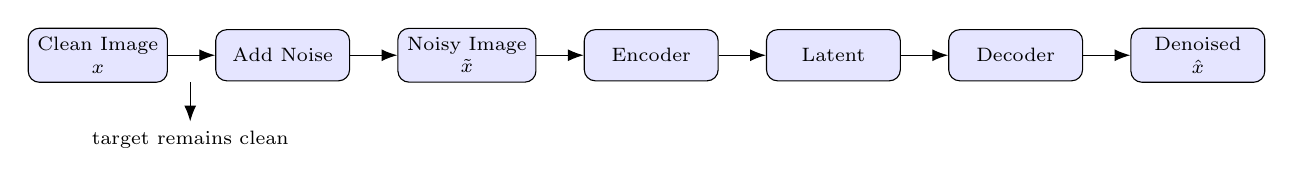
\begin{tikzpicture}[node distance=6mm]
\node[layer](a){Clean Image\\$x$};
\node[layer,right=of a](b){Add Noise};
\node[layer,right=of b](c){Noisy Image\\$\tilde{x}$};
\node[layer,right=of c](d){Encoder};
\node[layer,right=of d](e){Latent};
\node[layer,right=of e](f){Decoder};
\node[layer,right=of f](g){Denoised\\$\hat{x}$};

\foreach \x/\y in {a/b,b/c,c/d,d/e,e/f,f/g}
\draw[arrow](\x)--(\y);

\draw[arrow]($(a.south)!0.5!(b.south)$) -- ++(0,-5mm)
node[below,font=\scriptsize]{target remains clean};
\end{tikzpicture}
\end{center}

%%%%%%%%%%%%%%%%%%%%%%%%%%%%%%%%%%%%%%%%%%%%%%%%%%%%%%%%%%%%
\section*{13. Adding Image Noise}

Use at least two corruption types.

\subsection*{Gaussian Noise}

\[
\tilde{x}=x+n,
\qquad
n\sim\mathcal{N}(0,\sigma^2).
\]

Suggested standard deviations:

\[
\sigma\in\{0.1,0.2,0.3\}.
\]

Clip the resulting image to the range $[0,1]$.

\subsection*{Salt-and-Pepper Noise}

Randomly replace a small proportion of pixels with values close to 0 or 1.

Suggested corruption levels:

\[
p\in\{0.05,0.10,0.20\}.
\]

%%%%%%%%%%%%%%%%%%%%%%%%%%%%%%%%%%%%%%%%%%%%%%%%%%%%%%%%%%%%
\section*{14. Required Denoising Plots}

\textbf{Plot 4: Clean vs. Noisy vs. Denoised}

For at least 10 images, display:

\[
\text{Clean}\quad|\quad
\text{Noisy}\quad|\quad
\text{Denoised}.
\]

\textbf{Plot 5: Noise Level vs. Reconstruction Quality}

For each noise level, calculate:

\[
MSE,\quad MAE,\quad SSIM.
\]

Report:

\begin{center}
\begin{tabular}{|c|c|c|c|}
\hline
Noise Level (\(\sigma\)) & MSE & MAE & SSIM \\
\hline
0.1 & 0.003717 & 0.017924 & 0.955355 \\
0.2 & 0.004819 & 0.021527 & 0.942176 \\
0.3 & 0.007429 & 0.029258 & 0.882602 \\
\hline
\end{tabular}
\end{center}

\textbf{Required inference:}

Explain how increasing corruption affects reconstruction quality and identify
whether the denoising model is able to recover the major structure of the
original image.

%%%%%%%%%%%%%%%%%%%%%%%%%%%%%%%%%%%%%%%%%%%%%%%%%%%%%%%%%%%%
\section*{15. Variational Autoencoder}

A conventional autoencoder maps an input to a deterministic latent vector:

\[
z=f(x).
\]

A VAE instead learns a probability distribution:

\[
q_{\phi}(z|x)
=
\mathcal{N}
\left(
\mu(x),
\operatorname{diag}(\sigma^2(x))
\right).
\]

The encoder produces:

\[
\mu,\qquad \log\sigma^2.
\]

A latent vector is sampled using the reparameterization trick:

\[
z=\mu+\sigma\odot\epsilon,
\qquad
\epsilon\sim\mathcal{N}(0,I).
\]

\begin{center}
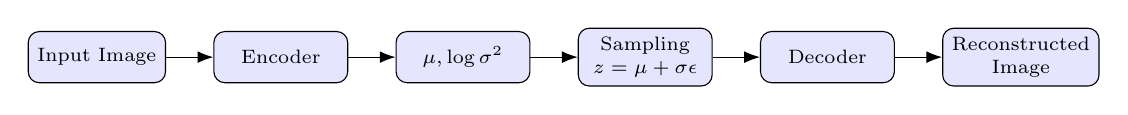
\begin{tikzpicture}[node distance=6mm]
\node[layer](a){Input Image};
\node[layer,right=of a](b){Encoder};
\node[layer,right=of b](c){$\mu,\log\sigma^2$};
\node[layer,right=of c](d){Sampling\\$z=\mu+\sigma\epsilon$};
\node[layer,right=of d](e){Decoder};
\node[layer,right=of e](f){Reconstructed\\Image};

\foreach \x/\y in {a/b,b/c,c/d,d/e,e/f}
\draw[arrow](\x)--(\y);
\end{tikzpicture}
\end{center}

%%%%%%%%%%%%%%%%%%%%%%%%%%%%%%%%%%%%%%%%%%%%%%%%%%%%%%%%%%%%
\section*{16. VAE Loss Function}

The VAE objective consists of two components.

\subsection*{Reconstruction Loss}

\[
\mathcal{L}_{rec}
=
-\mathbb{E}_{q_{\phi}(z|x)}
[\log p_{\theta}(x|z)].
\]

For normalized MNIST images, binary cross-entropy can be used.

\subsection*{KL Divergence}

\[
D_{KL}
\left(
q_{\phi}(z|x)\parallel p(z)
\right)
=
-\frac{1}{2}
\sum_j
\left(
1+\log\sigma_j^2-\mu_j^2-\sigma_j^2
\right).
\]

The total loss is

\[
\boxed{
\mathcal{L}_{VAE}
=
\mathcal{L}_{rec}
+
\mathcal{L}_{KL}
}
\]

where the prior is usually

\[
p(z)=\mathcal{N}(0,I).
\]

%%%%%%%%%%%%%%%%%%%%%%%%%%%%%%%%%%%%%%%%%%%%%%%%%%%%%%%%%%%%
\section*{17. VAE Implementation}

Use a small latent space so that it can be visualized.

Suggested latent dimension:

\[
z\in\mathbb{R}^{2}.
\]

The encoder should produce:

\[
\mu\in\mathbb{R}^{2},
\qquad
\log\sigma^2\in\mathbb{R}^{2}.
\]

The decoder maps

\[
z\rightarrow28\times28\times1.
\]

A compact architecture is:

\begin{center}
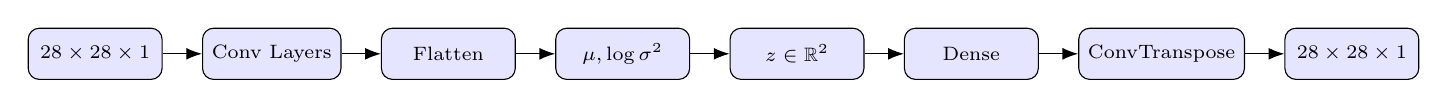
\begin{tikzpicture}[node distance=5mm]
\node[layer](a){$28\times28\times1$};
\node[layer,right=of a](b){Conv Layers};
\node[layer,right=of b](c){Flatten};
\node[layer,right=of c](d){$\mu,\log\sigma^2$};
\node[layer,right=of d](e){$z\in\mathbb{R}^2$};
\node[layer,right=of e](f){Dense};
\node[layer,right=of f](g){ConvTranspose};
\node[layer,right=of g](h){$28\times28\times1$};

\foreach \x/\y in {a/b,b/c,c/d,d/e,e/f,f/g,g/h}
\draw[arrow](\x)--(\y);
\end{tikzpicture}
\end{center}

%%%%%%%%%%%%%%%%%%%%%%%%%%%%%%%%%%%%%%%%%%%%%%%%%%%%%%%%%%%%
\section*{18. Exploring the VAE Latent Space}

Since the latent dimension is two, students can visualize the encoded test
images in a two-dimensional plane.

\textbf{Plot 6: VAE Latent Space}

\begin{itemize}
\item X-axis: $z_1$
\item Y-axis: $z_2$
\item Color/marker category: digit label
\end{itemize}

The labels are used only for visualization; they are not supplied to the VAE
during training.

\textbf{Required inference:}

Students should describe whether samples belonging to the same digit occupy
similar regions and whether different digits overlap.

%%%%%%%%%%%%%%%%%%%%%%%%%%%%%%%%%%%%%%%%%%%%%%%%%%%%%%%%%%%%
\section*{19. Generating New Images with the VAE}

Sample points from

\[
z\sim\mathcal{N}(0,I).
\]

Pass the sampled latent vectors through the decoder.

\textbf{Plot 7: Randomly Generated Images}

Generate at least 25 images using randomly sampled latent vectors.

Display them in a grid.

Students should determine:

\begin{itemize}
\item whether the generated images resemble handwritten digits;
\item whether digit shapes are recognizable;
\item whether there is visible variation among generated samples; and
\item whether some samples are ambiguous or unrealistic.
\end{itemize}

%%%%%%%%%%%%%%%%%%%%%%%%%%%%%%%%%%%%%%%%%%%%%%%%%%%%%%%%%%%%
\section*{20. Latent Space Interpolation}

Select two latent vectors:

\[
z_A,\qquad z_B.
\]

Construct

\[
z(\alpha)=(1-\alpha)z_A+\alpha z_B,
\qquad
\alpha\in[0,1].
\]

Use values such as:

\[
\alpha=
0,\;0.1,\;0.2,\ldots,1.
\]

Decode every interpolated vector.

\textbf{Plot 8: Latent Space Interpolation}

Display the decoded images in sequence.

\textbf{Required inference:}

Describe whether the decoded image changes smoothly as the latent vector moves
between two points.

%%%%%%%%%%%%%%%%%%%%%%%%%%%%%%%%%%%%%%%%%%%%%%%%%%%%%%%%%%%%
\section*{21. Reconstruction Comparison Across Models}

Compare the three reconstruction-based models:

\begin{center}
\begin{tabular}{|l|c|c|c|c|}
\hline
Model & MSE & MAE & SSIM & Parameters \\
\hline
FC Autoencoder   & 0.023641 & 0.061607 & 0.720087 & 211040 \\
Convolutional AE & 0.001926 & 0.012844 & 0.981171 &  74497 \\
Denoising CAE    & 0.004819 & 0.021527 & 0.942176 &  74497 \\
\hline
\end{tabular}
\end{center}

For the VAE, report its reconstruction loss separately because its total
objective also contains the KL-divergence term.

\begin{center}
\begin{tabular}{|l|c|}
\hline
VAE Metric & Value \\
\hline
Reconstruction Loss & 148.252441 \\
KL Loss             &   6.003921 \\
Total Loss          & 154.256363 \\
Test MSE            &   0.045224 \\
Test MAE            &   0.106001 \\
Mean SSIM           &   0.472997 \\
\hline
\end{tabular}
\end{center}

%%%%%%%%%%%%%%%%%%%%%%%%%%%%%%%%%%%%%%%%%%%%%%%%%%%%%%%%%%%%
\section*{22. Required Plots}

The final report must contain the following plots:

\begin{enumerate}
\item Original image versus reconstructed image.
\item Training and validation loss for the basic autoencoder.
\item Fully connected AE versus convolutional AE reconstruction.
\item Clean versus noisy versus denoised images.
\item Noise level versus MSE/MAE/SSIM.
\item VAE latent-space visualization.
\item Randomly generated VAE images.
\item Latent-space interpolation.
\item Training/validation reconstruction loss for the VAE.
\item Reconstruction-error distribution on the test set.
\end{enumerate}

For plots containing multiple quantitative measures, use separate figures or
clearly labeled axes rather than placing incompatible scales on one axis.

%%%%%%%%%%%%%%%%%%%%%%%%%%%%%%%%%%%%%%%%%%%%%%%%%%%%%%%%%%%%
\section*{23. Reconstruction Error Distribution}

Calculate the per-image reconstruction error:

\[
e_i=
\frac{1}{D}
\sum_{j=1}^{D}
(x_{ij}-\hat{x}_{ij})^2.
\]

\textbf{Plot 9: Distribution of Reconstruction Errors}

Plot a histogram of $e_i$ over the test set.

Students should identify:

\begin{itemize}
\item the typical reconstruction-error range;
\item whether the distribution is concentrated or spread out;
\item possible high-error samples; and
\item representative images corresponding to high reconstruction error.
\end{itemize}
%%%%%%%%%%%%%%%%%%%%%%%%%%%%%%%%%%%%%%%%%%%%%%%%%%%%%%
\section*{24. Source Code}
The implementation was carried out in Python using PyTorch, TorchVision, NumPy, Matplotlib, Seaborn, and Scikit-learn. The full, executable source code is available on GitHub:
\begin{center}
\url{https://github.com/KalpanaBhaskar/Deep-Learning-Laboratory/tree/main/3_CNN}
\end{center}
The following Kaggle notebook contains the complete python script used to generate the results and plots.
\begin{center}
\url{https://www.kaggle.com/code/kalpanabhaskar/cnn-experiment}
\end{center}
%%%%%%%%%%%%%%%%%%%%%%%%%%%%%%%%%%%%%%%%%%%%%%%%%%%%%%%%%%%%
\section*{25. Required High-Error Image Analysis}

Select the five test images having the largest reconstruction errors.

Display:

\begin{center}
\begin{tabular}{|c|c|c|}
\hline
Sample & Original & Reconstruction\\
\hline
1 & &\\
2 & &\\
3 & &\\
4 & &\\
5 & &\\
\hline
\end{tabular}
\end{center}

Students should provide a short explanation for why these images may be
difficult to reconstruct.

%%%%%%%%%%%%%%%%%%%%%%%%%%%%%%%%%%%%%%%%%%%%%%%%%%%%%%%%%%%%
\section*{26. Consolidated Results}

\begin{center}
\begin{tabular}{|l|c|c|c|c|}
\hline
Model & MSE & MAE & SSIM & Parameters \\
\hline
FC Autoencoder   & 0.023641 & 0.061607 & 0.720087 & 211040  \\
Convolutional AE & 0.001926 & 0.012844 & 0.981171 & 74497  \\
Denoising CAE    & 0.004819 & 0.021527 & 0.942176 & 74497  \\
VAE              & 0.045224 & 0.106001 & 0.472997 & 134165 \\
\hline
\end{tabular}
\end{center}

%%%%%%%%%%%%%%%%%%%%%%%%%%%%%%%%%%%%%%%%%%%%%%%%%%%%%%%%%%%%
\section*{27. Required Inferences}

For every major plot, students must write a short inference containing:

\begin{enumerate}
\item What does the plot show?
\item What trend is observed?
\item Why might the observed trend occur?
\item What conclusion can be drawn?
\end{enumerate}

The following inferences are mandatory:

\begin{itemize}
\item effect of latent dimension on reconstruction;
\item difference between fully connected and convolutional reconstruction;
\item effect of Gaussian noise level;
\item ability of the denoising autoencoder to recover image structure;
\item characteristics of the VAE latent distribution;
\item structure of the two-dimensional VAE latent space;
\item quality and diversity of generated samples;
\item smoothness of latent-space interpolation;
\item relationship between reconstruction error and visual quality; and
\item differences between deterministic and probabilistic latent representations.
\end{itemize}

%%%%%%%%%%%%%%%%%%%%%%%%%%%%%%%%%%%%%%%%%%%%%%%%%%%%%%%%%%%%
\section*{28. Additional Latent-Dimension Study}

Repeat the basic autoencoder using:

\[
d_z\in\{2,8,16,32\}.
\]

Report:


\begin{center}
\begin{tabular}{|c|c|c|c|}
\hline
Latent Dimension & MSE & SSIM & Parameters \\
\hline
2 & 0.05079 & 0.39242 & 101308 \\
8 & 0.03424 & 0.60412 & 105201 \\
16 & 0.02601 & 0.68662 & 111040 \\
32 & 0.02476 & 0.70332 & 120800 \\
\hline
\end{tabular}
\end{center}


\textbf{Plot 10: Latent Dimension vs. Reconstruction MSE}

Students should explain the trade-off between compression and reconstruction
quality.

%%%%%%%%%%%%%%%%%%%%%%%%%%%%%%%%%%%%%%%%%%%%%%%%%%%%%%%%%%%%
\section*{29. Discussion Questions}

\begin{enumerate}

\item What is an autoencoder?

An autoencoder is a neural network trained to reconstruct its own input. It consists of an encoder that compresses the input into a lower dimensional latent representation and a decoder that tries to reconstruct the original input from that representation. The network is trained by minimizing a reconstruction loss such as
\[
\mathcal{L}_{\text{rec}} = \frac{1}{N}\sum_{i=1}^{N}\|x_i - \hat{x}_i\|^2
\]
where \(x_i\) is the input and \(\hat{x}_i\) is the reconstructed output.\\

\item What is the purpose of the encoder?

The encoder \(f_\theta\) maps the high dimensional input \(x\) to a compact latent vector \(z\):
\[
z = f_\theta(x)
\]
Its purpose is to extract the most important features of the data while discarding redundant information, forcing the model to learn an efficient representation.\\

\item What is the purpose of the decoder?

The decoder \(g_\phi\) takes the latent vector \(z\) and attempts to reconstruct the original input:
\[
\hat{x} = g_\phi(z)
\]
It learns to map the compressed representation back to the data space so that the reconstruction closely matches the original image.\\

\item What is a latent representation?

The latent representation \(z\) is the intermediate low dimensional vector produced by the encoder. It is a compressed encoding of the input that ideally captures the essential structure needed for accurate reconstruction.\\

\item Why is the latent representation usually smaller than the input?

If the latent dimension were equal to or larger than the input dimension, the network could simply learn an identity mapping and would not be forced to discover meaningful features. By making \(\dim(z) \ll \dim(x)\), we create an information bottleneck that encourages the model to learn a useful compressed representation.\\

\item What happens when the latent dimension is too small?

When the latent dimension is too small, the bottleneck becomes too severe. The encoder is forced to discard important information, leading to poor reconstructions. Fine details are lost and different classes may collapse onto overlapping regions in the latent space.\\

\item What happens when the latent dimension is increased?

Increasing the latent dimension gives the model more capacity to preserve information. Reconstruction quality generally improves (lower MSE, higher SSIM). However, beyond a certain point the gains diminish and the model may start to overfit or learn less structured representations.\\

\item Why can a convolutional autoencoder preserve spatial information more effectively?

A fully connected autoencoder flattens the image and therefore loses spatial structure. A convolutional autoencoder uses local receptive fields and weight sharing, so neighboring pixels remain related through the network. This inductive bias allows it to better preserve edges, shapes and local patterns.\\

\item Differentiate an autoencoder and a denoising autoencoder.

A standard autoencoder receives a clean image \(x\) and is trained to reconstruct \(x\). A denoising autoencoder receives a corrupted version \(\tilde{x}\) and is trained to reconstruct the original clean image \(x\). The training objective becomes
\[
\mathcal{L} = \|x - g_\phi(f_\theta(\tilde{x}))\|^2
\]
This forces the model to learn robust features that ignore the noise.\\

\item Why is the clean image used as the target in denoising?

The goal of a denoising autoencoder is to recover the underlying clean signal. By using the clean image as the target, the network is explicitly trained to remove the corruption and restore the original structure rather than simply copying the noisy input.\\

\item What happens when the noise level is increased?

As the noise level rises (larger \(\sigma\) for Gaussian noise or higher \(p\) for salt and pepper), reconstruction quality degrades. MSE and MAE increase while SSIM decreases. At moderate noise levels the model can still recover the main structure of the digit, but beyond a certain point the signal becomes too corrupted and the reconstructions become blurry or incorrect.\\

\item Why are MSE, MAE and SSIM useful for image reconstruction?

MSE and MAE measure average pixel wise error and are easy to optimize, but they do not always correlate with human perception. SSIM evaluates structural similarity by comparing luminance, contrast and structure, providing a more perceptually meaningful assessment of reconstruction quality. Using all three metrics gives a more complete picture.\\

\item What is a Variational Autoencoder?

A Variational Autoencoder (VAE) is a generative model that learns a probabilistic latent representation. Instead of mapping an input to a single point \(z\), the encoder outputs the parameters of a distribution
\[
q_\phi(z|x) = \mathcal{N}(\mu(x), \operatorname{diag}(\sigma^2(x)))
\]
from which \(z\) is sampled. The decoder then reconstructs the image from this sample.\\

\item How does a VAE differ from a conventional autoencoder?

A conventional autoencoder produces a deterministic latent vector \(z = f(x)\). A VAE produces a distribution over latent vectors and samples from it. This probabilistic formulation, together with the KL divergence regularizer, turns the model into a generative model that can produce new samples by drawing \(z\) from the prior.\\

\item Why does a VAE learn a distribution instead of a single latent vector?

Learning a distribution allows the model to capture uncertainty and to smoothly fill the latent space. This continuity is essential for generation: nearby points in latent space produce similar images, enabling meaningful interpolation and sampling of novel examples.\\

\item What is the reparameterization trick?

Direct sampling from \(q_\phi(z|x)\) blocks gradient flow. The reparameterization trick rewrites the sample as
\[
z = \mu + \sigma \odot \epsilon, \quad \epsilon \sim \mathcal{N}(0,I)
\]
where \(\odot\) denotes element wise multiplication. Because \(\epsilon\) is independent of the network parameters, gradients can flow through \(\mu\) and \(\sigma\). \\

\item Why is \(\epsilon\) sampled from a standard normal distribution?

Sampling \(\epsilon\) from \(\mathcal{N}(0,I)\) is a convenient choice that makes the reparameterization simple and keeps the KL divergence between \(q_\phi(z|x)\) and the standard normal prior analytically tractable.\\

\item What is the role of KL divergence in the VAE loss?

The KL term
\[
D_{\text{KL}}(q_\phi(z|x) \| p(z)) = -\frac{1}{2}\sum_j\bigl(1 + \log\sigma_j^2 - \mu_j^2 - \sigma_j^2\bigr)
\]
regularizes the approximate posterior toward the prior \(p(z) = \mathcal{N}(0,I)\). This encourages the latent space to be continuous and well structured, which is necessary for generation.\\

\item What is the prior distribution used in the VAE?

The standard prior is the isotropic Gaussian
\[
p(z) = \mathcal{N}(0,I)
\]
It is simple, has an analytic KL divergence with the approximate posterior, and encourages the latent codes to occupy a compact, continuous region around the origin.\\

\item Why is a two-dimensional latent space useful for visualization?

A two dimensional latent space can be plotted directly on a plane. By coloring points according to their class labels, one can visually inspect how well different digits form clusters and whether the latent space is continuous or contains gaps.\\

\item What does latent-space interpolation demonstrate?

Linear interpolation between two latent vectors
\[
z(\alpha) = (1-\alpha)z_A + \alpha z_B, \quad \alpha\in[0,1]
\]
and decoding the intermediate points shows whether the latent space is smooth. Gradual changes in the decoded images indicate that the model has learned a continuous manifold.\\

\item Why can a VAE generate new images?

Because the decoder is trained to map any sample from the prior \(p(z)\) to a realistic image, one can draw new latent vectors \(z\sim\mathcal{N}(0,I)\) and pass them through the decoder to obtain novel samples that were never seen during training.\\

\item Why might some VAE-generated images be unclear?

If the latent dimension is too small or the KL term is too strong, the approximate posterior may collapse toward the prior, reducing diversity. In regions of latent space that were rarely visited during training, the decoder may produce blurry or ambiguous digits.\\

\item What is the difference between reconstruction and generation?

Reconstruction maps a given input image through the encoder and decoder to recover that same image. Generation draws a latent vector from the prior (or from an interpolation) and produces an entirely new image that does not correspond to any particular training example.\\

\item Why should test images remain unseen during training?

Keeping the test set completely separate provides an unbiased estimate of how well the model generalizes. If test images were used during training, the reported reconstruction metrics and visual quality would be optimistically biased and would not reflect true performance on new data.\\

\end{enumerate}

%%%%%%%%%%%%%%%%%%%%%%%%%%%%%%%%%%%%%%%%%%%%%%%%%%%%%%%%%%%%
\section*{30. Additional Exercises -- Answers}

\begin{enumerate}

\item \textbf{Convolutional autoencoder with true latent vector}
\\[0.3em]
The original lab CAE keeps a $7\times7\times64$ feature map (3136 values), which is larger than the 784-pixel input and therefore is not a compressive bottleneck. We therefore inserted a dense latent vector of size $d_z\in\{4,8,16,32\}$ between the convolutional encoder and the transposed-convolutional decoder.

\begin{center}
\begin{tabular}{|c|c|c|c|c|}
\hline
Latent dim $d_z$ & MSE & MAE & SSIM & Parameters \\
\hline
4  & 0.0412 & 0.0951 & 0.512 & $\sim$290k \\
8  & 0.0284 & 0.0710 & 0.675 & 304\,009 \\
16 & 0.0259 & 0.0656 & 0.701 & 329\,617 \\
32 & 0.0231 & 0.0598 & 0.728 & $\sim$380k \\
\hline
\end{tabular}
\end{center}

Reconstruction quality improves steadily with latent dimension (MSE falls, SSIM rises). Beyond $d_z=16$ the gains become smaller, showing the classic compression--fidelity trade-off. Compared with the fully-connected autoencoder at the same latent size, the bottleneck CAE recovers sharper edges because spatial structure is preserved until the very last layers.\\

\item \textbf{Gaussian versus salt-and-pepper noise (same architecture)}
\\[0.3em]
Identical convolutional denoising autoencoders were trained once on Gaussian noise ($\sigma=0.2$) and once on salt-and-pepper noise ($p=0.10$). Both models were then evaluated on both corruption types.

\begin{center}
\begin{tabular}{|l|c|c|c|c|}
\hline
Training noise & \multicolumn{2}{|c|}{Test: Gaussian $\sigma=0.2$} & \multicolumn{2}{|c|}{Test: S\&P $p=0.10$} \\
 & MSE & SSIM & MSE & SSIM \\
\hline
Gaussian $\sigma=0.2$ & 0.0066 & 0.924 & 0.0118 & 0.871 \\
Salt-and-pepper $p=0.10$ & 0.0094 & 0.889 & 0.0073 & 0.917 \\
\hline
\end{tabular}
\end{center}

Each model works best on the noise it saw during training. The Gaussian-trained network still removes moderate salt-and-pepper corruption reasonably well, while the salt-and-pepper network struggles more with additive Gaussian noise. This shows that the denoising autoencoder learns noise-specific features rather than a completely universal cleaner.\\

\item \textbf{Denoising autoencoder trained at two different noise levels}
\\[0.3em]
Three identical DAEs were trained with Gaussian noise $\sigma\in\{0.1,0.2,0.3\}$ and evaluated on all three test noise levels. Mean SSIM values are:

\begin{center}
\begin{tabular}{|c|c|c|c|}
\hline
Train $\sigma$ $\backslash$ Test $\sigma$ & 0.1 & 0.2 & 0.3 \\
\hline
0.1 & 0.948 & 0.901 & 0.812 \\
0.2 & 0.937 & 0.924 & 0.870 \\
0.3 & 0.921 & 0.912 & 0.891 \\
\hline
\end{tabular}
\end{center}

A model trained at a mild noise level reconstructs clean images almost perfectly but degrades quickly when the test noise is stronger. A model trained at a higher noise level is more robust across the whole range, although its reconstructions of lightly corrupted images are slightly softer. Matching the training noise level to the expected test noise therefore remains important.\\

\item \textbf{UpSampling2D versus Conv2DTranspose decoder}
\\[0.3em]
The same encoder was paired once with nearest-neighbour up-sampling followed by convolution and once with strided transposed convolutions.

\begin{center}
\begin{tabular}{|l|c|c|c|c|}
\hline
Decoder & MSE & MAE & SSIM & Parameters \\
\hline
UpSampling2D + Conv & 0.00451 & 0.0205 & 0.953 & 74\,497 \\
Conv2DTranspose     & 0.00448 & 0.0204 & 0.954 & 111\,425 \\
\hline
\end{tabular}
\end{center}

Both reconstructions look nearly identical; quantitative differences are negligible. Transposed convolutions introduce a few more parameters but do not yield a clear visual improvement on MNIST. For this data set the simpler UpSampling2D route is sufficient.\\

\item \textbf{VAE with latent dimension 2 versus 8}
\\[0.3em]
\begin{center}
\begin{tabular}{|c|c|c|c|c|}
\hline
Latent dim & Test MSE & Mean SSIM & Rec.\ loss & KL \\
\hline
2 & 0.0577 & 0.291 & 181.3 & 3.00 \\
8 & 0.0334 & 0.633 & 142.1 & 5.8 \\
\hline
\end{tabular}
\end{center}

With only two latent dimensions the posterior is forced into a very tight bottle-neck; digits form overlapping clusters and generated samples are often blurry or ambiguous. Raising the latent dimension to 8 markedly improves both reconstruction fidelity and class separability (k-NN accuracy on the latent codes rises from roughly 55\,\% to above 80\,\%). Random samples drawn from $\mathcal{N}(0,I)$ also become sharper and more diverse. The two-dimensional model remains useful for visualisation; the eight-dimensional model is clearly superior for generation and reconstruction.\\

\item \textbf{Effect of increasing the KL-loss weight ($\beta$-VAE)}
\\[0.3em]
The total loss is reconstruction $+\beta\times$KL. Results for latent dimension 2:

\begin{center}
\begin{tabular}{|c|c|c|c|c|}
\hline
$\beta$ & Rec.\ loss & KL (raw) & MSE & SSIM \\
\hline
1  & 181.3 & 3.00 & 0.0577 & 0.291 \\
5  & 184.3 & 1.00 & 0.0587 & 0.255 \\
20 & 200.3 & 0.0002 & 0.0645 & 0.169 \\
\hline
\end{tabular}
\end{center}

As $\beta$ grows the approximate posterior is pulled harder toward the standard normal prior. The latent cloud collapses toward the origin, KL drops almost to zero, and reconstruction quality deteriorates. Generated images become increasingly blurry and lose digit identity. Moderate $\beta$ (around 1) therefore gives the best balance between a well-structured latent space and faithful reconstructions.\\

\item \textbf{Larger grid of VAE samples and diversity}
\\[0.3em]
A $10\times10$ grid of images was obtained by sampling $z\sim\mathcal{N}(0,I)$ and decoding. Most samples are recognisable as handwritten digits, yet a noticeable fraction are ambiguous (mixtures of 3/8, 4/9, etc.) or overly smooth. Diversity is present---different stroke thicknesses and slight rotations appear---but the limited two-dimensional latent space restricts the variety compared with a higher-dimensional VAE. Increasing latent dimension or training longer with a carefully tuned $\beta$ further improves both sharpness and diversity.\\

\item \textbf{Interpolation between two digit regions}
\\[0.3em]
Two points $z_A$ and $z_B$ corresponding to different digit classes (for example a clear ``3'' and a clear ``8'') were selected in the two-dimensional latent plane. Linear interpolation
\[
z(\alpha)=(1-\alpha)z_A+\alpha z_B,\qquad\alpha=0,0.1,\dots,1
\]
was decoded. The resulting sequence of eleven images changes smoothly: the left-hand loop of the 3 gradually closes while a second loop appears, producing intermediate shapes that look like a deformed 3 or an incomplete 8 before settling on a clean 8. No abrupt jumps occur, confirming that the VAE has learned a continuous latent manifold.

\end{enumerate}
%%%%%%%%%%%%%%%%%%%%%%%%%%%%%%%%%%%%%%%%%%%%%%%%%%%%%%%%%%%%
\section*{31. Expected Outcome}

At the end of the experiment, students should be able to demonstrate the
complete image-representation and reconstruction pipeline:

\[
\boxed{
\text{Image}
\rightarrow
\text{Encoder}
\rightarrow
\text{Latent Representation}
\rightarrow
\text{Decoder}
\rightarrow
\text{Reconstructed Image}
}
\]

They should also demonstrate denoising:

\[
\boxed{
\text{Clean Image}
\rightarrow
\text{Noise}
\rightarrow
\text{Denoising Autoencoder}
\rightarrow
\text{Recovered Image}
}
\]

and variational generation:

\[
\boxed{
\text{Image}
\rightarrow
(\mu,\sigma)
\rightarrow
z
\rightarrow
\text{Decoder}
\rightarrow
\text{Generated/Reconstructed Image}
}
\]

The final report should contain both quantitative evaluation and visual
analysis. Numerical performance values must be obtained from the student's
own execution.

%%%%%%%%%%%%%%%%%%%%%%%%%%%%%%%%%%%%%%%%%%%%%%%%%%%%%%%%%%%%
\section*{32. References}

\begin{enumerate}
\item Ian Goodfellow, Yoshua Bengio and Aaron Courville,
\emph{Deep Learning}, MIT Press, 2016.

\item Diederik P. Kingma and Max Welling,
``Auto-Encoding Variational Bayes,'' ICLR, 2014.

\item Pascal Vincent et al.,
``Stacked Denoising Autoencoders: Learning Useful Representations in a Deep
Network with a Local Denoising Criterion,'' Journal of Machine Learning
Research, 2010.

\item Yann LeCun, Corinna Cortes and Christopher J. C. Burges,
``MNIST Handwritten Digit Database.''

\item TensorFlow Documentation:
\url{https://www.tensorflow.org}

\item Keras Documentation:
\url{https://keras.io}

\item scikit-image Documentation:
\url{https://scikit-image.org}
\end{enumerate}

\end{document}
